\begin{figure}[H]
    \centering
    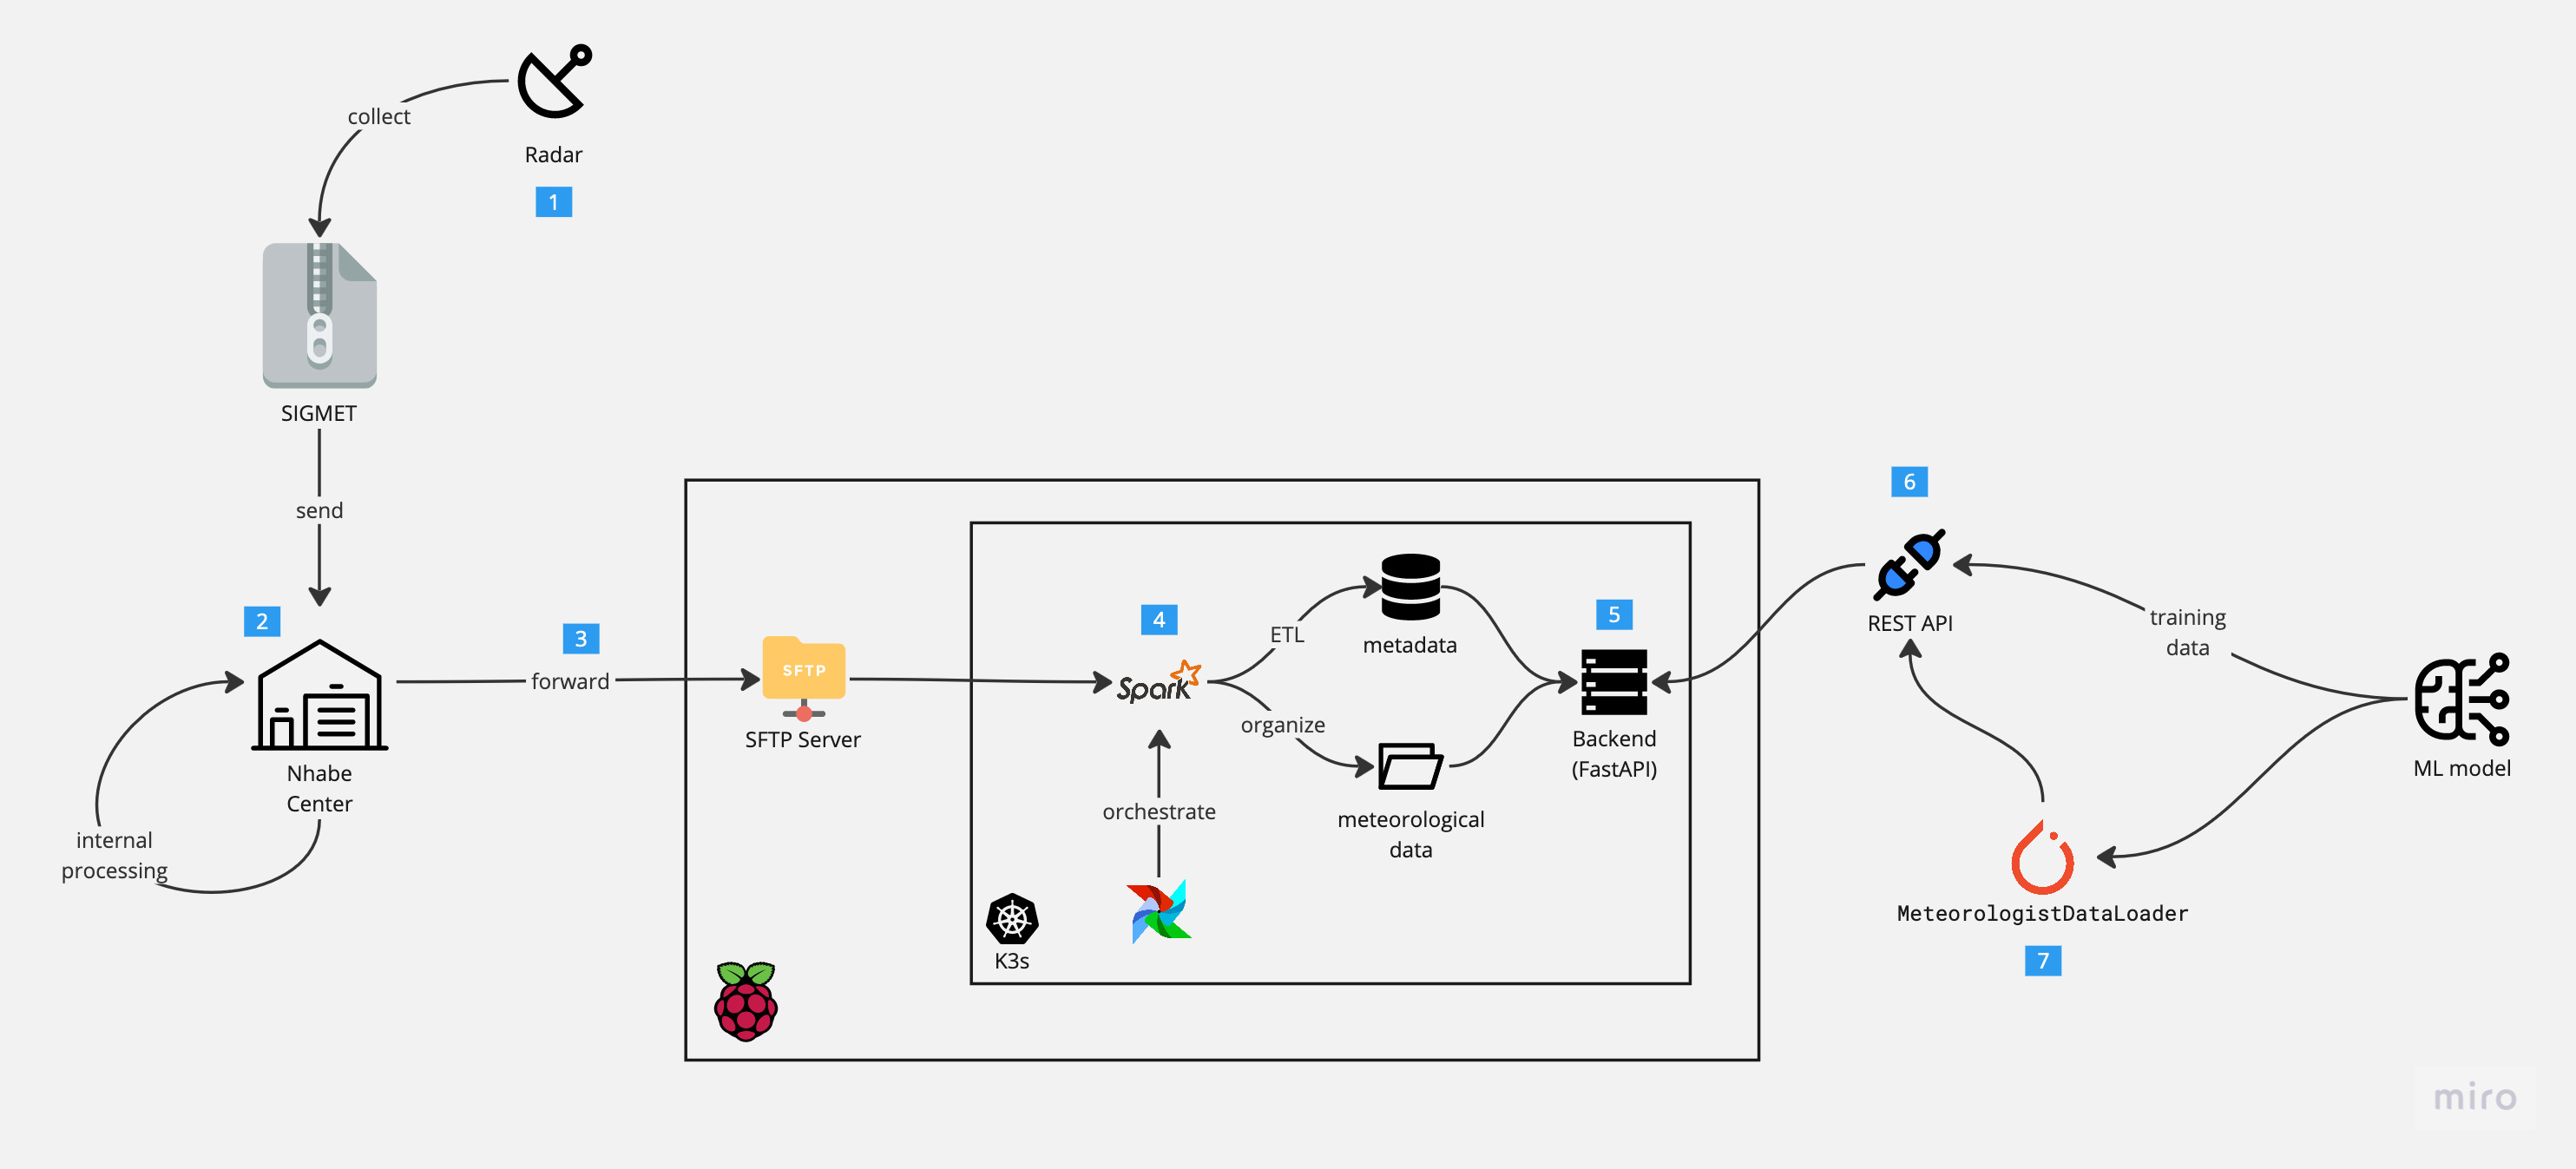
\includegraphics[width=1.05\linewidth]{Images/4.1-architecture.jpg}
    \vspace{1em}
    \caption{Thiết kế hệ thống - đề xuất}
    \label{fig:sow}
\end{figure}
\vspace{0.5cm}
Dựa vào những yêu cầu đặt ra từ các bên liên quan, cũng như sau khi được tìm hiểu về hệ thống hiện tại, nhóm đề xuất thiết kế và hiện thực một hệ thống "Cơ sở dữ liệu tích hợp cho hệ thống dự đoán ngắn hạn trong Khí tượng thuỷ văn". Hình \ref{fig:sow} minh hoạ cho mẫu thiết kế của nhóm.
\newpage
\section{Hệ thống hiện tại}
Nội dung thiết kế gồm 7 phần chính. Trong đó, phần hệ thống đang trong quá trình hoạt động tại trạm quan trắc Nhà Bè được thể hiện ở hai bước đầu tiên:

Trước tiên, tại bước 1, trong mỗi chu kỳ nhất định, vệ tinh địa tĩnh sẽ thu nhập dữ liệu về khí tượng. Một số những chỉ số thu nhận được có thể kể đến như:
\begin{enumerate}
    \item Độ rộng phổ Doppler (Doppler spectrum width)
    \item Tốc độ gió Doppler trung bình (Mean doppler velocity)
    \item Phản hồi vô tuyến (Reflectivity)
\end{enumerate}

Tất cả những thông tin này sẽ được truyền về trạm quan trắc tại Nhà Bè dưới định dạng SIGMET \ref{sigmet}. Sau đó, ở bước 2, những nhân viên tại trạm khí tượng thuỷ văn Nhà Bè sẽ tiến hành ghi nhận và xử lý các dữ liệu được truyền về, tuỳ theo các yêu cầu về nghiệp vụ của họ.

